%!TEX TS-program = pdflatex

\documentclass[12pt]{article}
\usepackage{amsfonts, amsmath, amssymb}
\usepackage{dcolumn, multirow}
\usepackage{setspace}
\usepackage{graphicx}
\usepackage{tabularx}
\usepackage{anysize, indentfirst, setspace}
\usepackage{verbatim, rotating, paralist}
\usepackage{latexsym}
\usepackage{amsthm}
\usepackage{parskip}
\usepackage{hyperref}
\usepackage{color}
\usepackage[right=2.5cm, left=2.5cm, top=3.5cm, bottom=3.5cm]{geometry} %right=, left=, top=, bottom=

\title{Estimate the Impact of Opioid Control Policies}
\author{Mid-Semester Project, Practical Data Science 1}
\date{\today}

\begin{document}
\maketitle

\subsection*{Background}

Over the past two decades, the United States has seen a tremendous increase in the use and abuse of prescription opioids, leading not only to a huge rise in opioid addiction, but also a rise in prescription overdose deaths, and increasingly deaths from non-prescription opioids like heroin and fentanyl as people who became addicted to opioids due to prescriptions turn to illegal markets to sustain their addiction.

\begin{figure}[h!]
  \centering
  \caption{Opioid Epidemic}\label{}
  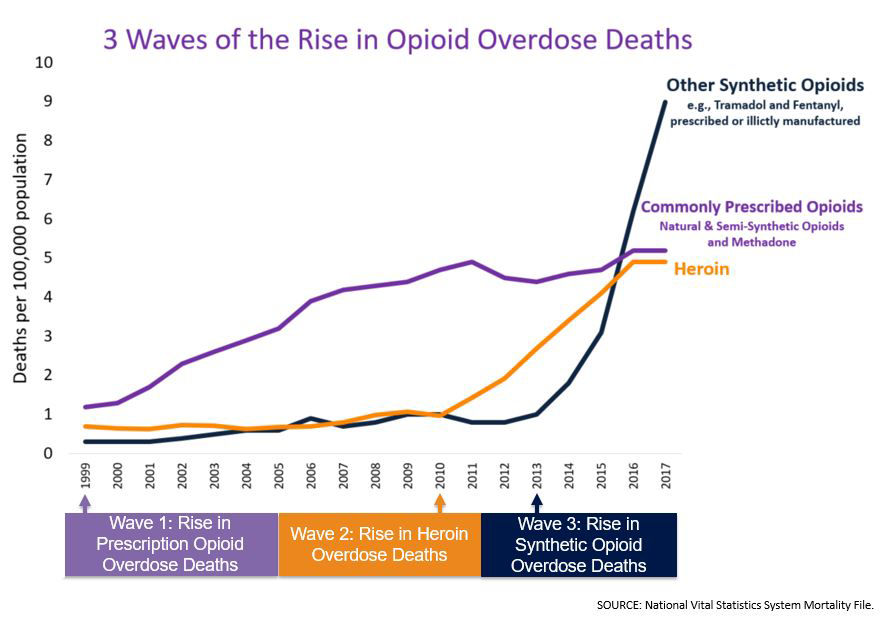
\includegraphics[width=0.6\textwidth]{images/cdc_opioid_stats.png}\\
  \scriptsize{Source: US Centers for Disease Control}
\end{figure}

In this project, we'll be \textbf{estimating the effectiveness of policy interventions} designed to limit the over-prescription of opioids. More specifically, we will attempt to measure the effect of a series of policy changes designed to limited opioid abuse in several US states on (a) opioid drug prescriptions, and (b) mortality from drug overdoses.\footnote{ In particular, we will focus on a Texas regulation that went into effect in January 2007, a Washington regulation that went into effect in January of 2012, and a Florida regulation that went into effect in 2010.}

Our interest in examining mortality as well as opioid prescriptions comes from the fact that while restricting access to opioids may reduce the likelihood that \emph{future} patients will end up addicted to opioids, it may drive already addicted patients to turn to alternative forms of opioids, be those illegally purchased prescription drugs, heroin, or fentanyl. This possibility is deeply troubling because the likelihood of overdosing on these illegal drugs is \emph{much} higher than on prescription drugs, as it is impossible for drug users to know the strength of illegal drugs, and because drugs like fentanyl are so potent that as little as 3mg can be lethal.

While our substantive focus is on opioid prescribing regulations, however, it is worth noting that in many ways you can see this as a template for policy evaluations more broadly. This is a specific application of an approach to measuring the impact of a policy, not a novel approach to analyzing opioid regulation.

\subsection*{The Question}

The goal of this project is to answer the following question: what is the effect of opioid drug prescription regulations on

\begin{enumerate}
  \item the volume of opioids prescribed,
  \item prescription opioid overdose deaths, and
  \item overdose deaths from non-prescription opioids (e.g. heroin, fentanyl)
\end{enumerate}

\subsection*{What An Answer Looks Like}

In developing a data science project, it is good practice to \emph{start} by asking what an answer to your question will look like. Once you know what you are trying to achieve, one can then work backwards to figure out what data will be needed to answer the question, what data manipulations will be required, and how you can divide those tasks among teammates.

In this case, the question we are asking is a \emph{causal question}, meaning that we are interested in understanding the \emph{effect} of one thing on another (i.e. what is the \emph{effect} of X on Y).

In a magical, idealized world, the way we would answer a causal question is to create two world: one in which our causal factor (here, a specific policy change) takes place, and one where it does not. Then we can say ``how did things turnout differently for Florida in 2010 in the world with the policy change \emph{as compared to the world where no policy change took place in Florida in 2010.}''

In the real world, however, we can never actually see both a world with the policy change and a world without the policy change for the same unit of observation. In the language of causal inference, we can never directly observe our \emph{counter factual} (Florida \emph{without} a policy change in 2010) -- we only get to see Florida with the policy change in 2010.\footnote{This is what is referred to as the Fundamental Problem of Causal Inference.}

With that in mind, we have to find a way to \emph{estimate} what we think \emph{would} have happened in Floria had there been no policy change. And this, in a nutshell, is the art of causal inference.

There are many approaches to solving this problem. The one we're most familiar with is randomized drug trials, where we randomly assign people to either take a drug or not take a drug. In these designs, the theory is that because people are being randomly assigned to take the drug or not, by the law of large numbers we expect the people who take the drug to be, on average, the same as the people who don't take the drug. Because of these, we \emph{assume} that what happens to the people who aren't taking the drug is, \emph{on average}, what \emph{would} have happened to the people do are taking the drug \emph{if they hadn't taken the drug}. In other words, we think that the non-drug-takers are a good counter-factual for the drug takers.

(If this is making your head spin a little, don't worry -- this stuff is hard, and this is a very quick intro to causal inference. About half of my Spring course will be focused on these ideas.)

But we can't randomly assign states to either or not implement opioid control measures, so we need to come up with different ways of estimating what we think would have happened to Florida had it not passed opioid control measures.

\subsubsection*{Pre-Post Comparison}

One of the most basic strategies, and the one we'll use first, is to compare how things were in Florida right before the policy went into effect to Florida right after the policy went into effect. In doing so, we're assuming that had the opioid policy not gone into effect, Florida in 2011 would have looked more or less like it looked in 2009.

This type of analysis would likely come out with a result that looks something like this:

\begin{figure}
  \centering
  \caption{}\label{}
  %\includegraphics{}
  If volume reduced  \hspace{1cm} If volume not reduced
\end{figure}

\subsubsection*{Difference-in-Difference}

A simple pre-post comparison is a good, simple approach to causal inference, but it is not without its problems.

Suppose, for example, that around 2010 (the same time Florida's policy went into effect) the US Customs service managed to dramatically reduce the importation of fentanyl into the United States. This would likely reduce the amount of overdose deaths throughout the United States, and so if we were just comparing Florida in 2009 to Florida in 2011, we would see a decline in overdose deaths and wrongly attribute that to Florida's policy change.

One strategy for dealing with this is what's called a \emph{difference-in-difference} approach. In simple terms, we don't just compare Florida in 2009 to Florida in 2011; instead, we ask ``were there bigger changes in overdose deaths in Florida between 2009 and 2011 \emph{than in other states that didn't change their opioid policy}?'' If Florida's policy had an effect, then we would expect opioid overdoses in Florida to decrease differently from in states without a policy change. But if Florida experienced a decline in overdoses because of something that happened nationally (e.g. if US Customs blocked opioid importation), then we'd expect to see overdoses reduce at the same rate in all states.

In other words, was the change we saw in Florida (the ``difference'' from pre-to-post) larger than the change that occurred in other states? Or, to map this onto the term ``difference-in-difference,'' if we estimate the \emph{difference} between 2009 and 2011 separately for Florida and states without policy changes, is there a difference in those differences?

This type of analysis generates a result that looks like this:

\begin{figure}
  \centering
  \caption{}\label{}
  %\includegraphics{}
  If volume reduced  \hspace{1cm} If volume not reduced
\end{figure}

https://azdhs.gov/documents/prevention/womens-childrens-health/injury-prevention/opioid-prevention/

[regression]

\subsection*{Data}

Two sources of data you will definitely need for this analysis are information on (a) opioid prescriptions, and (b) drug overdose mortality. Sources for this data are provided below. You will also likely need at least one other source of data, which you will be required to find on your own.

\subsubsection*{Opioid Prescriptions}

A core component of this project will be a recently released dataset of all prescription opioid drug shipments in the United States from 2006 to 2012. This was only \emph{just} released (in mid-2019) by the \emph{Washington Post}, which obtained the data through a Freedom of Information Act (FOIA) request to the US Drug Enforcement Agency.

\begin{itemize}
  \item \href{https://www.washingtonpost.com/graphics/2019/investigations/dea-pain-pill-database/}{Read about data here.}
  \item \href{https://www.washingtonpost.com/national/2019/07/18/how-download-use-dea-pain-pills-database/?arc404=true}{Download here.}
\end{itemize}

\subsubsection*{Mortality Data}

The best national source of data on drug overdoses is the US Vital Statistics records, which include data on every death in the United States. You can find information about the Vital Statistics and download data \href{https://www.cdc.gov/nchs/nvss/deaths.htm}{here}.


\subsection*{Unit of Observation}

A big part of any data science project is figuring out your \emph{unit of observation.} Your choice of unit of observation is dictated not just by what is theoretically appropriate, but also what is feasible given the data available. You may \emph{want} to study a question with individual-level data, but if you can only get data that is aggregated at the level of cities, you don't have the option of working at the individual-level.

As many students doing this project are not Americans and so are unlikely to be familiar with US administrative districting, I will spare you the challenge of figuring out the right geographic unit of analysis for this project: the geographic unit of analysis we'll be working are counties (though you get to figure out the appropriate temporal unit yourself!).

Counties are administrative units in the US that fall entirely \emph{within} states, but with can otherwise vary in about any way they want. In some states, like North Carolina, counties are relatively regular in size (as shown in the Figure~\ref{counties} below), though they often vary radically in population (in North Carolina, county populations vary from over 1 million people (Mecklenberg and Wade Counties) to well under 10,000 (Hyde and Tyrrell Counties)). In other states, like Colorado (also pictured below), some counties (like Denver, a little above and to the right of the center of the state) are much smaller than other counties geographically.

\begin{figure}[h!]
  \centering
  \caption{US County Maps}\label{counties}
  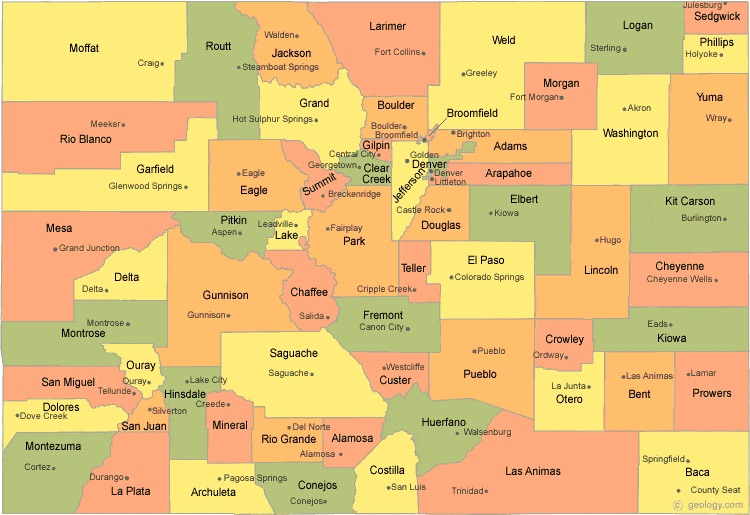
\includegraphics[width=0.4\textwidth]{images/CO_counties.jpg}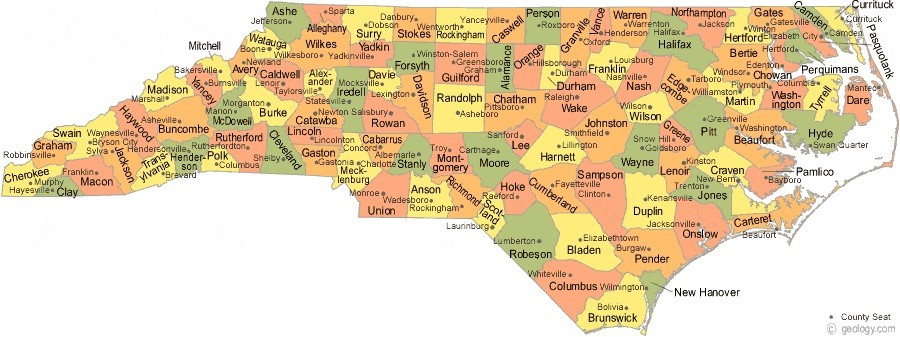
\includegraphics[width=0.4\textwidth]{images/NC_counties.jpg}\\
  \scriptsize{Colorado \hspace*{5cm} North Carolina}
\end{figure}

What they are kind of odd in terms of their heterogeneity, however, they are common units of analysis for US government data because they are more granular than states, but also big enough that reporting the number of deaths from drug overdoses in a given county doesn't threaten the privacy of individuals. And indeed, in this analysis, we will find that all our data is available at \emph{at least} the county level.

Things to know about counties:

\begin{itemize}
  \item Counties vary dramatically in population and geographic size
  \item County names are \emph{not} unique across states. The same county name will appear in many states.
  \item All US counties and states have assigned numeric identifiers called ``FIPS codes.'' Not all datasets will include county's FIPS codes, but if you can find them, they're much easier to use than county names since you don't have to worry about capitalizations and such. You can find datasets online easy that will tell you the FIPS code for a given county given its state and name.
\end{itemize}

\subsection*{Policy Changes}

In this analysis, we'll be analyzing \emph{three} policy changes:

\begin{itemize}
  \item Texas, Effective January 4, 2007
  \begin{itemize}
    \item ``In 2007, the Texas Medical Board adopted regulations with regards to treating pain with
controlled substances. The guidelines include performing a patient evaluation before prescribing opioids (including reviewing
prescription data and history related to the patient contained in the state’s prescription drug monitoring program (PDMP)), obtaining informed consent from the patient for opioid treatment, conduct periodic review of the opioid treatment, and maintain a complete medical record of the patient’s treatment.''\footnote{Source: The Network for Public Health Law, \href{https://azdhs.gov/documents/prevention/womens-childrens-health/injury-prevention/opioid-prevention/appendix-b-state-by-state-summary.pdf}{Appendix B}}. \href{https://texreg.sos.state.tx.us/public/readtac$ext.TacPage?sl=R&app=9&p_dir=&p_rloc=&p_tloc=&p_ploc=&pg=1&p_tac=&ti=22&pt=9&ch=170&rl=3}{Link to law.}
  \end{itemize}
  \item Florida, Effective February, 2010
  \begin{itemize}
    \item ``Florida gained notoriety after 2007 because of the proliferation of pain clinics in the state that were prescribing large quantities of drugs for pain with little medical justification and were being used primarily by persons abusing or diverting opioid analgesics, benzodiazepines, and muscle relaxants. In 2010, Florida was also home to 98 of the 100 U. S. physicians who dispensed the highest quantities of oxycodone directly from their offices. In response, Florida enacted several measures to address prescribing that was inconsistent with best practices. The Florida legislature required that pain clinics treating pain with controlled substances register with the state by January 4, 2010. In February 2010, the Drug Enforcement Administration and various Florida law enforcement agencies began to work together in Operation Pill Nation. Pain clinic regulations were further expanded later in 2010. In February 2011, law enforcement conducted statewide raids, resulting in numerous arrests, seizures of assets, and pain clinic closures. In July of that year, coinciding with a public health emergency declaration by the Florida Surgeon General, the state legislature prohibited physician dispensing of schedule II or III drugs from their offices and activated regional strike forces to address the emergency. Mandatory dispenser reporting to the newly established prescription drug monitoring program began in September 2011. Finally, in 2012, the legislature expanded regulation of wholesale drug distributors and created the Statewide Task Force on Prescription Drug Abuse and Newborns.''\footnote{Source: Johnson, Paulozzi, Porucznik, Mack, and Herter, 2014.} \textbf{Note:} Obviously what we have here is a \emph{series} of changes rather than one single large change. Nevertheless, for this analysis just operationalize the policy change as having taken place in February 2010.
  \end{itemize}
  \item Washington (the State, not Washington, DC), Effective Jan 2, 2012.
  \begin{itemize}
    \item In 2011, the Washington Department of Health adopted a rule regulating the prescribing of opioids for pain treatment. Some of the prescribing requirements include:\footnote{Source: The Network for Public Health Law, \href{https://azdhs.gov/documents/prevention/womens-childrens-health/injury-prevention/opioid-prevention/appendix-b-state-by-state-summary.pdf}{Appendix B}}
    \begin{itemize}
      \item For patients who are stable involving non-escalating daily doses of 40 mg MED/day or less, periodic reviews shall take place annually.
      \item Mandatory consultation threshold for adults is 120 mg MED/day (oral).
      \item In the event a physician prescribes a dosage that meets or exceeds the consultation
      threshold, a consultation with a pain management specialist is required.
      \item The physician shall document each mandatory consultation.
      \item Recommended that a practitioner not prescribe more than an average of MED of
      120 mg without either the patient demonstrating improvement in function or without first obtaining a consultation from a pain management expert.
    \end{itemize}
    \item \href{http://apps.leg.wa.gov/documents/laws/wsr/2011/12/11-12-025.htm}{Link to regulation.}
    \end{itemize}
\end{itemize}


\subsection*{Your Task}

Your task is to complete a pre-post analysis and a difference-in-difference analysis of these three policy changes. You can present your results in the graphical format modeled above. While there are many statistical methods of doing things like adding controls for various observable factors, the emphasis on this analysis is on data wrangling and transparent analysis, so those plots will be sufficient.

For this project, you must:

\begin{itemize}
  \item Gather all data needed to complete this analysis
  \item Clean, organize, and merge it in order to allow for creation of the final analysis.
  \item Do all your work transparently through github \emph{as a team}.
  \begin{itemize}
    \item All team members must make substantial commits to the project.
    \item All team members must also actively review at least one PR for another team member.
  \end{itemize}
  \item Present a final report that summarizes in your own words:
  \begin{itemize}
    \item The motivation for the project,
    \item The motivation for the research design being used,
    \item Details of the data used and how different datasets have been related to one another,
    \item Your analysis,
    \item Your interpretation of that analysis.
  \end{itemize}
  In writing you report, you should assume that the person reading your report is policy maker with \emph{limited} statistical training. That means you should strive to limit the use of jargon wherever possible.
  \item A preliminary draft of your report will be due November [X]
  \item A final draft of your report will be due November [X]
\end{itemize}

\end{document}
